% +++
% latex="lualatex"
% +++
\documentclass[aspectratio=149,9pt,fleqn,tbtags]{beamer}
\usetheme[numbering=fraction,block=fill]{metropolis}
\usefonttheme{professionalfonts}

\setbeamersize{text margin left=1em,text margin right=1em}

\usepackage{luatexja,luatexja-adjust}
\usepackage[no-math,match,deluxe]{luatexja-fontspec}

\hypersetup{unicode,colorlinks}
\hypersetup{linkcolor=blue,urlcolor=teal,citecolor=olive}
% \hypersetup{linkcolor=black,urlcolor=black,citecolor=black}

\usepackage{pxrubrica}
\usepackage{autobreak}
\usepackage{tikz,pgfplots,tcolorbox}
\usetikzlibrary{calc}
\pgfplotsset{compat=1.16}

\usepackage[version=4,arrows=pgf]{mhchem}
\mhchemoptions{textfontcommand=\sffamily,mathfontcommand=\mathsf}
\newcommand*\cec[1]{\cesplit{{\,\ }{\0}}{#1}}

\usepackage{array,booktabs,tabularray,subfigure}
\SetTblrDefault{rowsep=2pt}
\UseTblrLibrary{booktabs}

\usepackage[loadonly,]{enumitem}
\newlist{desc}{description}{5}
\setlist[desc]{labelindent=2\zw,labelsep*=1\zw,labelwidth=3\zw}
\newlist{enu}{enumerate}{5}
\setlist[enu]{label*=\arabic*.}

\ltjsetparameter{jacharrange={-2,-3,-8}}
\usepackage[no-math,match,deluxe,fontspec]{luatexja-preset}

% \usepackage[osf]{newpxtext}\usepackage{classico}
\usepackage[nowidering]{yhmath}
\usepackage{newpxmath,amsmath,mathtools,amssymb,mleftright}
\usepackage[T1]{fontenc}
\usepackage[notrig,italicdiff]{physics}
\mleftright

\usepackage[scr=boondoxo,frak=pxtx,bb=mth]{mathalfa}
\DeclareMathAlphabet{\mathnormal}{T1}{pplx}{m}{it}
\DeclareMathAlphabet{\mathrm}{T1}{pplx}{m}{n}
\DeclareMathAlphabet{\mathit}{T1}{pplx}{m}{it}
\DeclareMathAlphabet{\mathtt}{T1}{lmtt}{m}{n}
\DeclareMathAlphabet{\mathsf}{T1}{kurier}{m}{n}
\DeclareMathAlphabet{\mathbsf}{T1}{kurier}{b}{n}
\DeclareMathAlphabet{\mathbold}{T1}{pplx}{b}{it}
\DeclareMathAlphabet{\mathbf}{T1}{pplx}{b}{n}
\DeclareMathAlphabet{\mathscr}{U}{BOONDOX-calo}{m}{n}
\DeclareMathAlphabet{\mathbscr}{U}{BOONDOX-calo}{b}{n}
%\DeclareMathAlphabet{\mathcal}{OT1}{eusm10}{m}{n}
%\DeclareMathAlphabet{\mathbcal}{OT1}{eusm10}{b}{n}
\DeclareMathAlphabet{\mathfrak}{OT1}{tx-frak}{m}{n}
\DeclareMathAlphabet{\mathbfrak}{OT1}{tx-frak}{b}{n}
\DeclareMathAlphabet{\mathbb}{U}{dsss}{m}{n}
\DeclareSymbolFont{operators}{T1}{uop}{m}{n}

\DeclareSymbolFont{numbers}{T1}{pplx}{m}{n}
\DeclareMathSymbol{0}\mathalpha{numbers}{`0}
\DeclareMathSymbol{1}\mathalpha{numbers}{`1}
\DeclareMathSymbol{2}\mathalpha{numbers}{`2}
\DeclareMathSymbol{3}\mathalpha{numbers}{`3}
\DeclareMathSymbol{4}\mathalpha{numbers}{`4}
\DeclareMathSymbol{5}\mathalpha{numbers}{`5}
\DeclareMathSymbol{6}\mathalpha{numbers}{`6}
\DeclareMathSymbol{7}\mathalpha{numbers}{`7}
\DeclareMathSymbol{8}\mathalpha{numbers}{`8}
\DeclareMathSymbol{9}\mathalpha{numbers}{`9}

\DeclareFontFamily{U}{mathastro}{}
\DeclareFontShape{U}{mathastro}{m}{n}{<->mathastrotest10}{}
\DeclareSymbolFont{astro}{U}{mathastro}{m}{n}
\DeclareMathSymbol\Sun\mathord{astro}{'300}
\DeclareMathSymbol\Mercury\mathord{astro}{'301}
\DeclareMathSymbol\Venus\mathord{astro}{'302}
\DeclareMathSymbol\Earth\mathord{astro}{'303}
\DeclareMathSymbol\Mars\mathord{astro}{'304}
\DeclareMathSymbol\Jupiter\mathord{astro}{'305}
\DeclareMathSymbol\Saturn\mathord{astro}{'306}
\DeclareMathSymbol\Uranus\mathord{astro}{'307}
\DeclareMathSymbol\Neptune\mathord{astro}{'310}
\DeclareMathSymbol\Pluto\mathord{astro}{'311}
\DeclareMathSymbol\varEarth\mathord{astro}{'312}
\DeclareMathSymbol\Moon\mathord{astro}{'313}
\DeclareMathSymbol\leftmoon\mathord{astro}{'313}
\DeclareMathSymbol\rightmoon\mathord{astro}{'314}
\DeclareMathSymbol\fullmoon\mathord{astro}{'315}
\DeclareMathSymbol\newmoon\mathord{astro}{'316}
\DeclareMathSymbol\newmoon\mathord{astro}{'316}

\setmainfont[
	Ligatures=TeX,
	Scale=0.98,
	BoldFont=FOT-RodinNTLGPro-B,
	ItalicFont=FOT-RodinNTLGPro-B,
]{Palatino}
\setsansfont[
	Ligatures=TeX,
	Scale=0.98,
	BoldFont=FOT-RodinNTLGPro-B,
	BoldItalicFont=FOT-RodinNTLGPro-B,
	%ItalicFont=FOT-RodinNTLGPro-B,
]{Palatino}
\setmainjfont[
	Ligatures=TeX,
	JFM=jlreq,
	BoldFont=FOT-RodinNTLGPro-B,
	ItalicFont=FOT-RodinNTLGPro-B,
]{FOT-ModeMinBLargePro-M}
\setsansjfont[
	Ligatures=TeX,
	JFM=jlreq,
	BoldFont=FOT-RodinNTLGPro-B,
	ItalicFont=FOT-RodinNTLGPro-B,
]{FOT-ModeMinBLargePro-M}
\setmonofont[
	Ligatures=TeXReset,
]{HackGen}
\setmonojfont[
	Ligatures=TeXReset,
]{HackGen}

\allowdisplaybreaks[4]
\ltjenableadjust[lineend=extended,priority=true,profile=true,linestep=false]

%%%%%%%%%%%%自作マクロ
\newcommand{\hmvec}{\mathbold}
\newcommand{\hmeqdef}{\stackrel{\mathrm{def}}{=}}
\newcommand{\hmeqq}{\stackrel{\mathrm{?}}{=}}
\newcommand{\centeralign}[1]{\rule{0pt}{0pt}\hfill#1\hfill\rule{0pt}{0pt}}
\NewDocumentCommand\hmu{s m}{\IfBooleanF{#1}{\,}\ifmmode\mathrm{#2}\else\(\mathrm{#2}\)\fi}
\newcommand{\hmemph}[1]{\textbf{#1}}
\newcommand{\hme}[1]{\times10^{#1}}
\newcommand{\hmfnc}[1]{\(\mathrm{#1}\)}
\newcommand{\hmfconv}{F_\mathrm{conv}}
\newcommand{\jp}[1]{{\footnotesize #1}}
\NewDocumentCommand\etal{s}{\textit{et al.}\IfBooleanF{#1}{\ }}

\institute{Planetary and Space Group\\北海道大学大学院理学院 宇宙理学専攻 地球流体力学研究室}
\author{Shoma Hitomi\\人見祥磨}
\title{Dependence of Atmospheric Meridional Heat Transports\\in Aqua Planets on Solar Constant}
\subtitle{水惑星における大気南北熱輸送の太陽定数依存性}

\begin{document}

\maketitle

\begin{frame}
	\frametitle{Introduction/背景}
	\begin{columns}[T]
		\begin{column}{.6\textwidth}
			\begin{itemize}
				\item The runaway greenhouse state is an important concept for
					understanding the variety of climates of the terrestrial planets.\\
					\jp{暴走温室状態は地球型惑星の気候を考察する上で重要な概念}
				%\item In this state, oceans will evaporate.\\
				%	\jp{暴走温室状態になると海洋が全て蒸発すると考えられる}
				\item One-dimensional radiative-convective equilibrium gray atmosphere models
					show the existence of upper limit of outgoing longwave radiation (OLR)
					(Nakajima \etal 1992).\\
					\jp{灰色 1 次元モデルでは外向き赤外放射 (OLR) に上限がある(射出限界)}
				\item The runaway greenhouse state is a state with incoming solar radiation
					greater than the upper limit.\\
					\jp{射出限界以上に入射があるのが暴走温室状態}
				\item A three-dimentional model also have upper limit of OLR.
					For solar radiation greater than the upper limit, the runaway
					greenhouse state appears (Ishiwatari \etal 2002).\\
					\jp{灰色 3 次元モデルでも OLR に上限が現れる}
			\end{itemize}
		\end{column}
		\begin{column}{.35\textwidth}
			\centering\scriptsize
			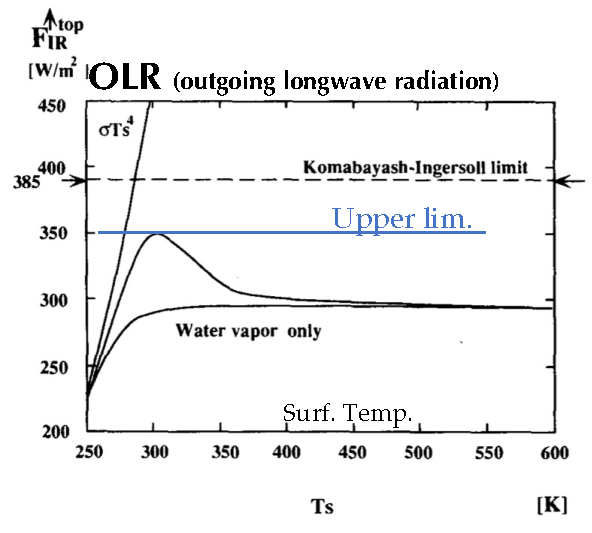
\includegraphics[width=.9\textwidth]{fig-n1992.pdf}\\
			The relationship between surface temp.~and OLR\\
			(Nakajima \etal*, 1992, Fig.~3)
			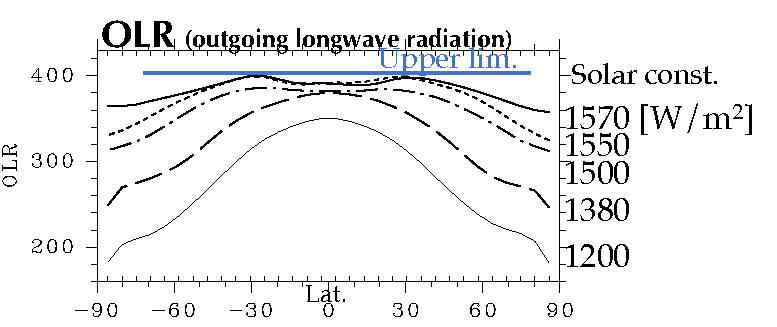
\includegraphics[width=\textwidth]{fig-i2002-olr.pdf}
			The meridional distributions of zonal mean OLR\\
			(Ishiwatari \etal*, 2002; Fig.~4a)
		\end{column}
	\end{columns}
\end{frame}

\begin{frame}
	\frametitle{Purpose/研究目的}
	\begin{itemize}
		\item Decrease of meridional thermal contrast gives upper limit of OLR in three-dimentional models.\\
			\jp{3 次元モデルで射出限界が決まったのは南北差の減少の影響が大きかった}
			\begin{itemize}
				%\item The runaway greenhouse state is caused in gray atmospheric three-dimentional models.\\
				%	\jp{3 次元でも暴走温室状態が起きうる}
				%\item Increasing solar constant cause meridional thermal contrast of zonal mean of OLR and
				%	surface temp.~decrease in gray atmospheric three-dimentional models.\\
				%	\jp{灰色 3 次元モデルでは、太陽定数を大きくすると OLR や地表面温度の南北差が小さくなる}
				\item Interpretations in one-dimentional models can be applied
					in three-dimentional models because meridional contrast is decreased.\\
					\jp{3 次元系では、高温になると南北差が小さくなるので、1 次元系の解釈を適用できる}
				\item The increase of solar constant cuases the increase of meriodinal heat transport
				%\item Increasing solar constant cause latent energy transports increases
				%	in gray atmospheric three-dimentional models.\\
					\jp{灰色 3 次元モデルでは太陽定数が大きくなると南北熱輸送が大きくなっていた}
			\end{itemize}
		\item However, Ishiwatari \etal (2002) use idealized model.
			What happens in more Earth-like situation?\\
			\jp{Ishiwatari \etal (2002) は非常に理想化されているが、より地球に近い状況ではどうなるのか考察する}
		\begin{itemize}
			\item e.g. non-gray atmospheric cloud-included situation.\\
				\jp{具体的な設定としては、非灰色大気、雲ありの設定}
		\end{itemize}
	\item In this study, I examine what happen when solar constant increases.\\
		\jp{太陽定数が大きくなったときに、どのようなことが起きているか考察する}
		\begin{itemize}
			\item Do meridional thermal contrast also decrease
				in non-gray atmospheric model when solar constant increases?\\
				\jp{非灰色大気でも太陽定数が大きくなったら南北一様化が起きるのか}
			\item If meridional thermal contrast decrease,
				how meridional heat transports happen?\\
				\jp{南北差が小さくなるならば、どのような南北熱輸送が起きているのか}
		\end{itemize}
	\end{itemize}
\end{frame}

\begin{frame}
	\frametitle{Methods/手法}
	\small
	\begin{columns}
		\begin{column}{.55\textwidth}
			\begin{itemize}
				\item Model/利用したモデル
					\begin{itemize}
						\item Atmospheric global circulation model (DCPAM5)/大気大循環モデル DCPAM 5\\
							{\footnotesize\url{http://www.gfd-dennou.org/library/dcpam/}}
					\end{itemize}
				\item Basic equations/基礎方程式
					\begin{itemize}
						\item 3-D primitive equations for a spherical geometry\\
							\jp{3 次元球殻領域のプリミティブ方程式}
					\end{itemize}
			\end{itemize}
			\tiny
			\begin{gather}
				\pdv{\pi}{t}+\vb*{v}_H\cdot\nabla_\sigma\pi=-D-\pdv{\dot \sigma}{\sigma},\tag{Continuity equation}\\
				\pdv{\Phi}{\sigma}=-\frac{RT_v}{\sigma},\tag{Hydrostatic equilibrium}\\
				\pdv{\zeta}{t}=\frac{1}{a}\qty(\frac{1}{1-\mu^2}\pdv{V_A}{\lambda}
					-\pdv{U_A}{\mu})+\mathcal{D}[\zeta],\tag{EOM1}\\
				\pdv{D}{t}=\frac{1}{a}\qty(\frac{1}{1-\mu^2}\pdv{U_A}{\lambda})
				-\nabla^2_\sigma(\Phi+R\bar T\pi+KE)+\mathcal{D}[D],\tag{EOM2}\\
				\begin{split}
					\pdv{T}{t}=&-\frac{1}{a}\qty(\frac{1}{1-\mu^2}\pdv{UT'}{\lambda}
						+\pdv{VT'}{\mu})+T'D-\dot\sigma\pdv{T}{\sigma}\\
					&+\kappa T_v\qty(\pdv{\pi}{t}+\vb*{v}_H\cdot\nabla_\sigma\pi+\frac{\dot\sigma}{\sigma})
						+\frac{Q}{C_p}+\mathcal{D}[T]+\mathcal{D}'[\vb*{v}],
				\end{split}\tag{Thermodynamics}\\
				\pdv{q}{t}=-\frac{1}{a}\qty(\frac{1}{1-\mu^2}\pdv{U_q}{\lambda}+\pdv{V_q}{\mu})
				+qD-\dot\sigma\pdv{q}{\sigma}+S_q+\mathcal{D}[q].\tag{Water Vapor}
			\end{gather}
		\end{column}
		\begin{column}{.45\textwidth}
			\begin{itemize}
				\item Physical Process/物理過程
					\begin{itemize}
						\scriptsize
						\item Radiation prosess for East/{地球用放射過程}\\
							(Chou and Lee, 1996; Chou \etal*,1998)
						\item Turbulent mixing/{乱流混合}\\
							(Mellor and Yamada, 1982)
						\item Dry convection adjustment/{乾燥対流調節}\\
							(Manabe \etal*, 1965)
						\item Relaxed Arakawa--Schubert\\
							(Moorthi and Suarez, 1992)
					\end{itemize}
			\end{itemize}
			\begin{table}[b]
				\tiny
				\centering
				\begin{minipage}{\textwidth}
					\rule[0pt]{\textwidth}{\heavyrulewidth}\\%
					\begin{minipage}{.5\textwidth}
						\hfill
						\begin{tabbing}
							\hspace*{3\zw}\=\kill
							\(\varphi,\lambda\)\>Latitude and longitude\\
							\(\sigma\coloneqq p/p_s\)\quad\(\sigma\) coordinate height\\
							\(t\)\>Time\\
							\(\pi\coloneqq\ln[p_s]\)\\
							\(T\)\>Temperature\\
							\(q\)\>Specific humidity\\
							\(a\)\>Radius of planet\\
							\(f\)\>Coriolis parameter\\
							%\(\displaystyle\zeta\coloneqq\frac{1}{a}
							%	\qty(\frac{1}{1-\mu^2}\pdv{V}{\lambda}-\pdv{U}{\mu})\)\quad 渦度\\
							%\(\displaystyle D\coloneqq\frac{1}{a}
							%	\qty(\frac{1}{1-\mu^2}\pdv{U}{\lambda}+\pdv{V}{\mu})\)\quad 発散\\
							\(\zeta\)\>Vorticity\\
							\(D\)\>Divergence\\
							\(u,v\)\>Eastward, northward wind\\
							\((U,V)\coloneqq(u\cos\varphi,v\cos\varphi)\)\\
							\(KE\coloneqq(U^2+V^2)/(2(1-\mu^2))\)\\
							\(\Phi\coloneqq gz\)\quad Geopotential
							%\(\displaystyle\sigma\coloneqq\pdv{\sigma}{t}\equiv
							%	\pdv{\sigma}{t}+\frac{u}{a\cos\phi}\pdv{\sigma}{\lambda}
							%	+\frac{v}{a}\pdv{\sigma}{\phi}+\pdv{\sigma}{\sigma}\)\\
						\end{tabbing}
					\end{minipage}
					\hfill
					\begin{minipage}{.5\textwidth}
						\hfill
						\begin{tabbing}
							\hspace*{3\zw}\=\kill
							%\(\displaystyle U_A\coloneqq(\zeta+f)V-\dot\sigma\pdv{U}{\sigma}
							%	-\frac{RT'_v}{a}\pdv{\pi}{\lambda}+\mathcal{F}_\lambda\cos\phi\)\\
							%\(\displaystyle V_A\coloneqq-(\zeta+f)U-\dot\sigma\pdv{V}{\sigma}
							%	\frac{RT'_v}{a}(1-\mu^2)\pdv{\pi}{\mu}+\mathcal{F}_\phi\cos\phi\)\\
							%\(\displaystyle\vb*{v}_H\vdot\nabla_\sigma\pi\coloneqq
							%	\frac{U}{a(1-\mu^2)}\pdv{\theta}{\lambda}+\frac{V}{a}\pdv{\pi}{\lambda}\)\\
							%\(\displaystyle\nabla_\sigma^2\coloneqq\frac{1}{a^2(1-\mu^2)}\pdv[2]{}{\lambda}
							%	+\frac{1}{a^2}\pdv{}{\mu}\qty[(1-\mu^2)\pdv{}{\mu}]\)\\
							%\(\mathcal{D}[\zeta]\)\>渦度の水平発散とスポンジ層での散逸\\
							%\(\mathcal{D}[D]\)\>発散の水平発散とスポンジ層での散逸\\
							%\(\mathcal{D}[T]\)\>熱の水平拡散\\
							%\(\mathcal{D}[q]\)\>水蒸気の水平拡散\\
							\(\mathcal{D}\)\>Horizontal diffusion\\
							\(\mathcal{D}'[\vb*{v}]\)\>Frictional heat\\
							\(\mathcal{F}\)\>Small-scale movement process\\
							%\(\mathcal{F}_\lambda\)\>小規模運動過程(経度方向)\\
							%\(\mathcal{F}_\phi\)\>小規模運動過程(緯度方向)\\
							\(Q\)\>Heating\\
							\(S_q\)\>Water vapor source\\
							\(R\)\>Gas constant of dry air\\
							\(c_{pn}\)\>Specific heats\\
							\>at constant press.~of dry air\\
							\(\kappa\coloneqq R/c_{pn}\)\\
							\(\epsilon_v\)\>Water vapor moleculars\\
							\>weight ratio\\
							\(\bar T\)\>Temperature level\\
							\(T'\coloneqq T-\bar T\)\\
							\(T_v\coloneqq T(1+(\epsilon_v^{-1}-1)q)\)\\
							\(T'_v\coloneqq T_v-\bar T\)
						\end{tabbing}
					\end{minipage}\\
					\rule[0pt]{\textwidth}{\heavyrulewidth}
				\end{minipage}
			\end{table}
		\end{column}
	\end{columns}
\end{frame}

\begin{frame}
	\frametitle{Experimental design/実験設定}
	\begin{columns}[T]
		\begin{column}{.55\textwidth}
			\begin{itemize}
				\item Experimental design/実験設定
					\begin{itemize}
						\item Aqua Planet/水惑星
						\item Paramters/パラメータ
					\end{itemize}
			\end{itemize}
			\begin{table}
				\centering\tiny
				\begin{tblr}{ll}
					\toprule
					Parameters&Value\\
					\midrule
					Radius of planet&\(a=6.37\hme{7}\hmu{m}\)\\
					Rotation angular velocity&\(\omega=7.292\hme{-5}\hmu{/s}\)\\
					Gravitational acceleration&\(g=9.8\hmu{m/s^2}\)\\
					Gas constant of dry air&\(R_n=287.1\hmu{J/kg/K}\)\\
					Gas constant of water vapor&\(R_v=461.5\hmu{J/kg/K}\)\\
					Specific heat at constant press.~of dry air&\(c_{pn}=1004\hmu{J/kg/K}\)\\
					Specific heat at constant press.ure of water vapor&\(c_{pv}=1810\hmu{J/kg/K}\)\\
					Molecular weight of dry air&\(m_n=28.96\hme{-3}\hmu{kg/mol}\)\\
					Molecular weight of water vapor&\(m_v=18.02\hme{-3}\hmu{kg/mol}\)\\
					Latent heat of water vapor&\(L=2.50\hme{6}\hmu{J/kg}\)\\
					Albedo of ocean&\(A=0.1\)\\
					\bottomrule
				\end{tblr}
			\end{table}
		\end{column}
		\begin{column}{.45\textwidth}
			\begin{itemize}
				\item Initial state/初期状態
					\begin{itemize}
						\item Temp./温度一様 \(280\hmu{K}\)
						\item Specific Humidity/比湿一様 \(0\)
						\item Resting Atmosphere/静止大気
					\end{itemize}
				\item List of experimets/実験リスト
			\end{itemize}
			\begin{table}
				\centering\small
				\begin{tblr}{lccccc}
					\toprule
					Expt.~&{Solor\\const.\\\(S\ [\hmu*{W/m^2}]\)}
					&{Cloud\\lifetime\\\([\hmu*{s}]\)}&{Integrate\\time\\\([\text{year}]\)}\\
					\midrule
					S1366&1366&13500&41\\
					S1500&1500&13500&11\\
					S1600&1600&13500&11\\
					S1800&1800&13500&11\\
					S2000&2000&13500&21\\
					\bottomrule
				\end{tblr}
			\end{table}
		\end{column}
	\end{columns}
\end{frame}

\begin{frame}
	\frametitle{Result---Emargence of equilibrium stats/結果---平衡状態に達しているか}
	\begin{columns}[T]
		\begin{column}{.45\textwidth}
			\begin{itemize}
				\item The atmosphere reaches equilibrium states in S1366 to S1800,
					because OLR (outgoing longwave radiation)
					become equal to OSR (outgoing shortwave radiation).\\
					\jp{S1366 から S1800 までは OLR と OSR が一致して平衡状態になっている}
				\item For S2000, more integration seems to be necessary
					to determine whether the system reaches is equilibrium state.\\
					\jp{S2000 は積分期間を長くしなければ平衡状態になっているか判断できない}
			\end{itemize}
		\end{column}
		\begin{column}{.5\textwidth}
			\begin{figure}[t]
				\centering\scriptsize
				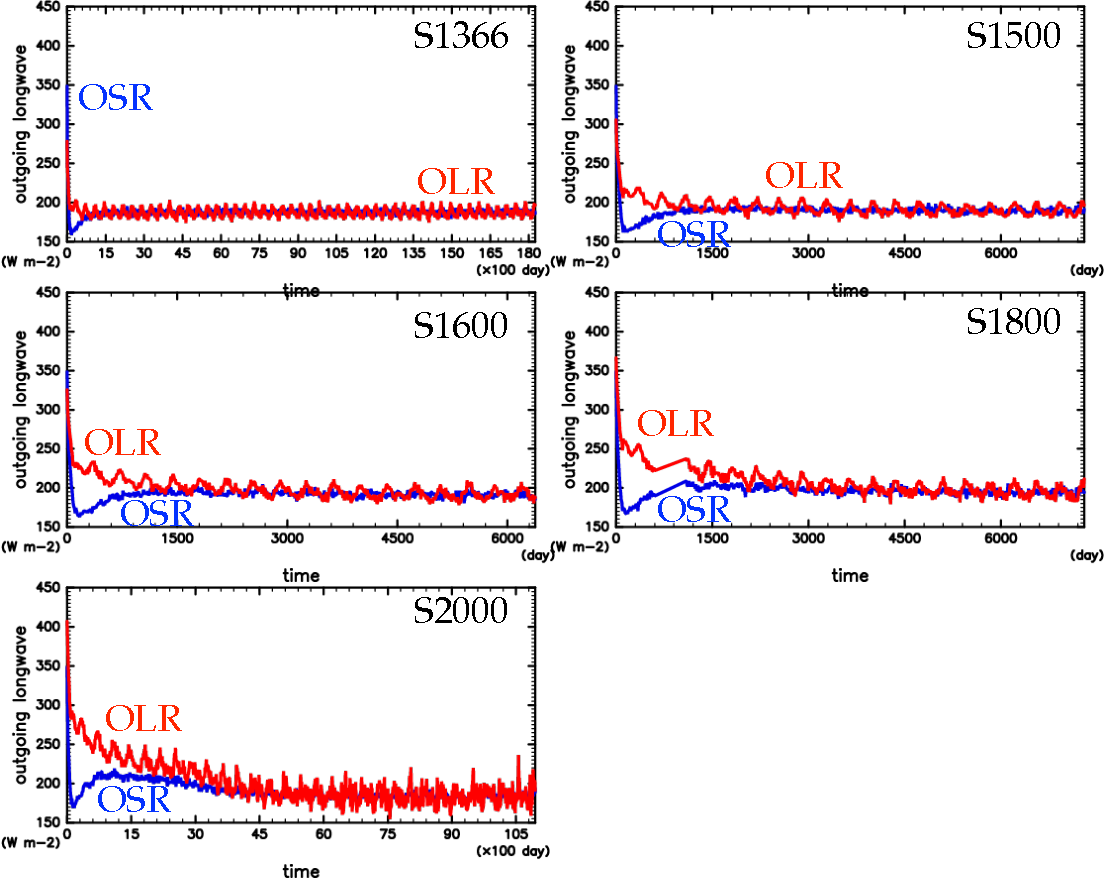
\includegraphics[width=\textwidth]{fig-osr-olr.pdf}
				Time evolutions of global mean OLR and OSR.
			\end{figure}
		\end{column}
	\end{columns}
\end{frame}

\begin{frame}
	\frametitle{Results---Decreaseing meridional thermal contrast/結果---南北差の減少}
	\begin{figure}
		\centering\footnotesize
		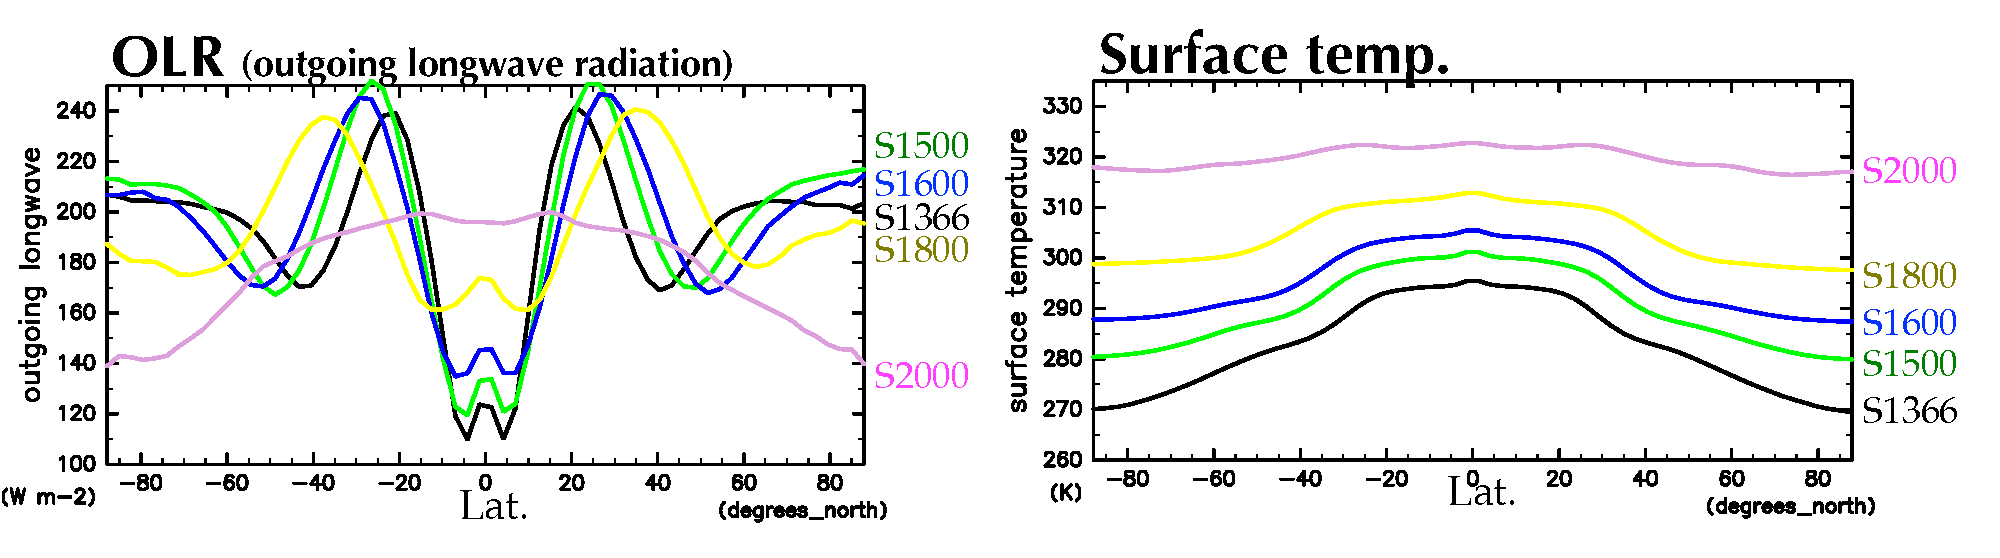
\includegraphics[width=.8\textwidth]{fig-osr-surftemp.pdf}\\
		Meridional distributions of zonal mean of OLR and surface temp.
	\end{figure}
	\begin{columns}[T]
		\begin{column}{\textwidth}
			\begin{itemize}
				\item Meridional contrasts of zonal mean OLR and surface tempraure
					decrease as solar constant increases in equilibrium state.\\
					\jp{非灰色大気でも太陽定数が増大すると OLR の東西平均と地表面温度の
					東西平均の南北差が小さくなる}
					\begin{itemize}
						\item OLR at the equator increases and OLR at mid-latitude
							decreases as solar constant increases.\\
							\jp{太陽定数の増大に従って、赤道の OLR は増加し、中緯度の OLR は減少する}
					\end{itemize}
			\end{itemize}
		\end{column}
	\end{columns}
\end{frame}

\begin{frame}
	\frametitle{Meridional heat transports/南北熱輸送}
	\begin{columns}[T]
		\begin{column}{\textwidth}
			\begin{itemize}
				\item Meridional energy transports \(F_T\) is written \(F_L+F_D\).\\
					\jp{南北方向の熱輸送 \(F_T\) は \(F_L+F_D\) と書ける}
					\begin{gather}
						F_T=F_L+F_D\notag\\
						F_L=\int_0^{2\pi}\int_0^{p_s} Lqv\,dp\,d\lambda,\tag{Latent energy}\\
						F_D=\int_0^{2\pi}\int_0^{p_s} (c_{pn}T+gz)v\,dp\,d\lambda.\tag{Dry static energy}
					\end{gather}
			\end{itemize}
		\end{column}
	\end{columns}
\end{frame}

\begin{frame}
	\frametitle{Results---Zonal time mean of meridional heat transports\\結果---南北熱輸送の東西時間平均}
	\begin{figure}
		\centering\scriptsize
		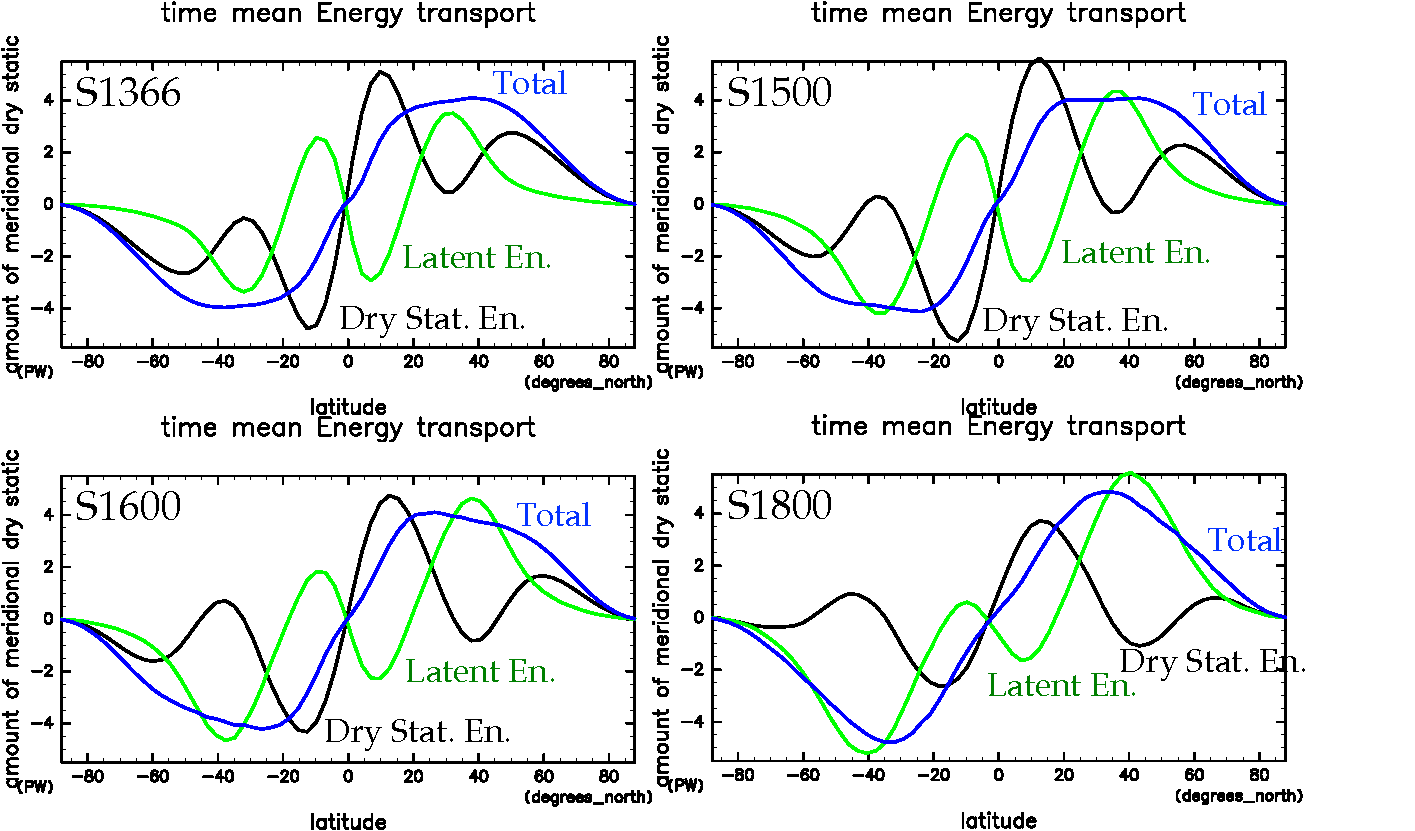
\includegraphics[width=.5\textwidth]{fig-enflx.pdf}
	\end{figure}
	\begin{columns}[T]
		\begin{column}{\textwidth}
			\begin{itemize}
				\item Total energy transport increases as solar constant is increased.
				\item Latent energy transport increases as solar constant is increased.\\
					\jp{南北熱輸送の合計と潜熱輸送は太陽定数が増大すると増大する}
				\item Dry static energy transport has maximun in S1500
					but increasing solar constant over S1600 cause decrease dry static energy flux.\\
					\jp{乾燥静的エネルギーの輸送は S1500 で最大になり、
					それ以降太陽定数が大きくなると小さくなる。}
			\end{itemize}
		\end{column}
	\end{columns}
\end{frame}

\begin{frame}
	\frametitle{Zonal time mean of latent energy and dry static energy\\
	各実験での潜熱と乾燥静的エネルギーの東西平均}
	\begin{figure}
		\centering\footnotesize
		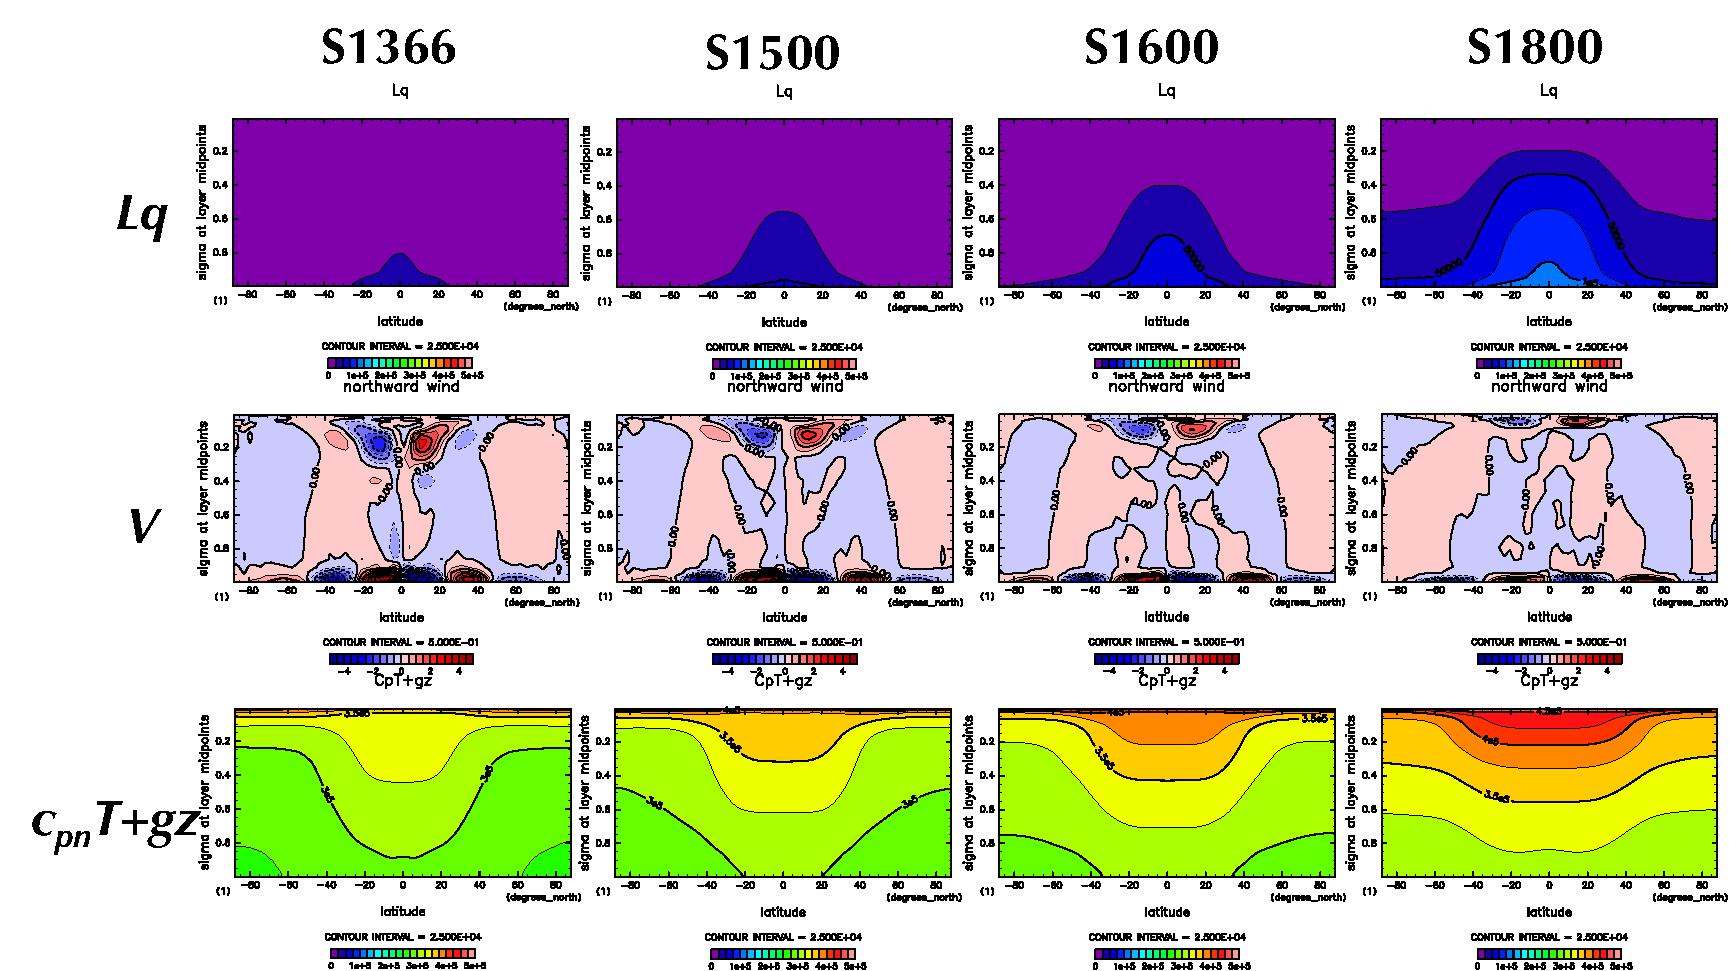
\includegraphics[width=.75\textwidth]{fig-cpt+gz.pdf}\\
	\end{figure}
	\begin{columns}[T]
		\begin{column}{\textwidth}
			\begin{itemize}
				\item Northward wind on upper atmosphere decrease as solar constant increases over S1600.
					This makes dry static energy transport decrease.\\
					\jp{S1600 以上では太陽定数が増大すると大気上層の
					南北風が小さくなるので乾燥静的エネルギーの輸送が小さくなる}
			\end{itemize}
		\end{column}
	\end{columns}
\end{frame}

\begin{frame}
	\frametitle{Next problem/現在取り組んでいる問題}
	\begin{columns}[T]
		\begin{column}{\textwidth}
			\begin{itemize}
				\item Disaggragate the transports three part.\\
					\jp{それぞれの輸送を次の 3 つによるものの和に分ける}
					\begin{gather}
						[\overline{xv}]=
						\underbracket{[\bar x][\bar v]}_{\text{mean meridional flow}}
						+\underbracket{[\bar{x^*}\bar{v^*}]}_{\text{stationary eddy}}
						+\underbracket{[\overline{x'v'}]}_{\text{transient eddy}}
						\quad\text{(\(x=Lq\) or \((c_{pn}T+gz))\)}.\notag
					\end{gather}
					\(\bar\bullet\): time mean; \([\bullet]\) zonal mean;
					\(\bullet'=\bullet-\bar\bullet, \bullet^*=\bullet-[\bullet]\): deviations from means
				\item I'm trying to figure out how each term affects the other.\\
					\jp{それぞれの項がどう影響しているか調べている}
					\begin{itemize}
						\item When solar constant is large, latent heat is transported
							by low and high pressure systems.\\
							\jp{太陽定数が大きいとき、潜熱輸送は低気圧・高気圧に依る部分が大きい}
						\item When solar consttabt is large, latent heat is transported
							by mean meridional flow.\\
							\jp{太陽定数が大きいとき、乾燥静的エネルギーの輸送は平均子午面の循環
							に依るところが大きい}
					\end{itemize}
			\end{itemize}
		\end{column}
	\end{columns}
\end{frame}

%\begin{frame}
%	\frametitle{結果---潜熱輸送の内訳/Results}
%	\begin{columns}[T]
%		\begin{column}{.5\textwidth}
%			\begin{itemize}
%				\item 停滞性擾乱による輸送はほぼない
%					\begin{itemize}
%						\item 地形がないため
%					\end{itemize}
%				\item 太陽定数が増大すると移動性擾乱による寄与が大きくなる
%			\end{itemize}
%		\end{column}
%		\begin{column}{.45\textwidth}
%			\begin{figure}
%				\centering\scriptsize
%				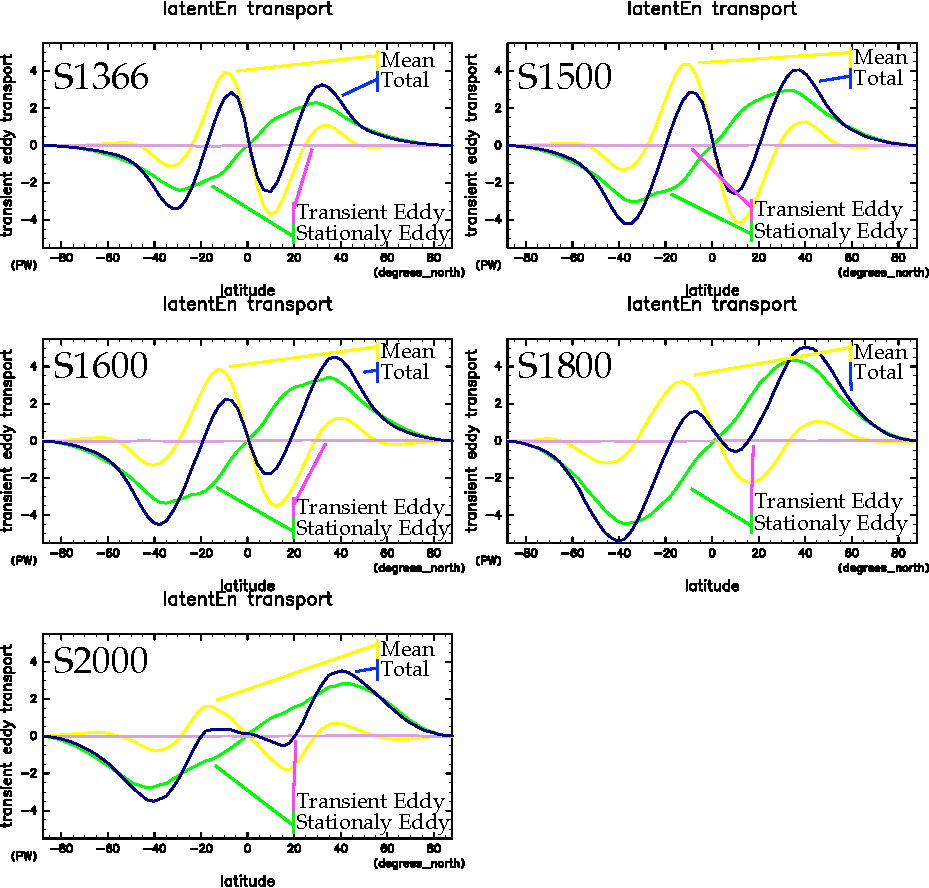
\includegraphics[width=\textwidth]{fig-latent.pdf}
%				各実験における潜熱輸送の内訳
%			\end{figure}
%		\end{column}
%	\end{columns}
%\end{frame}

%\begin{frame}
%	\frametitle{結果---乾燥静的エネルギー輸送の内訳/Results}
%	\begin{columns}[T]
%		\begin{column}{.5\textwidth}
%			\begin{itemize}
%				\item 先程示した南北輸送の図と一致してない(要検討)
%				\item 停滞性擾乱による輸送はほぼない
%					\begin{itemize}
%						\item 地形がないため
%					\end{itemize}
%				\item 太陽定数が増大すると平均子午面循環による輸送の寄与が大きくなる
%			\end{itemize}
%		\end{column}
%		\begin{column}{.45\textwidth}
%			\begin{figure}
%				\centering\scriptsize
%				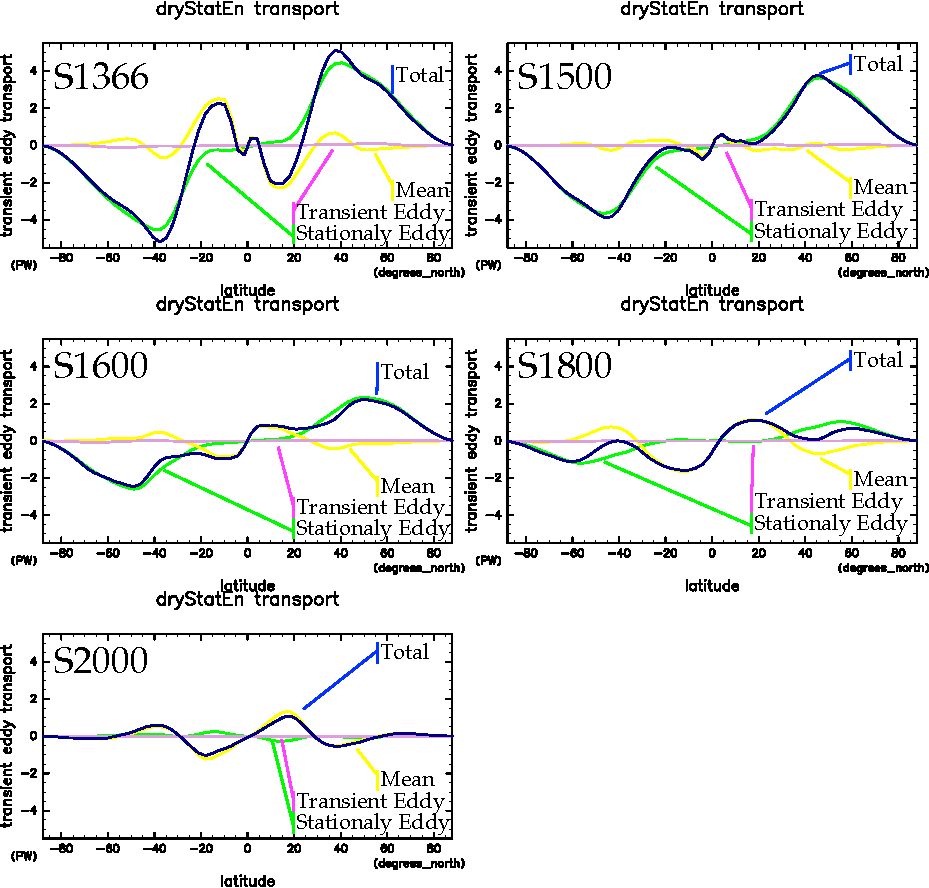
\includegraphics[width=\textwidth]{fig-drystat.pdf}
%				各実験における乾燥静的エネルギー輸送の内訳
%			\end{figure}
%		\end{column}
%	\end{columns}
%\end{frame}

\begin{frame}
	\frametitle{まとめ/Conclution}
	\begin{itemize}
		\item Dependence of atmospheric meridional heat transports
			on solar constant using three-dimentional spherical non-gray atmospheric model is examined.\\
			\jp{3 次元非灰色大気モデルで、太陽定数と南北熱輸送の関係を調べた}
		\item Increase of solar constant cause decrease of meridional thermal contrast.\\
			\jp{太陽定数が増大すると南北差が小さくなる}
		\item Increase of solar constant cause total meridional heat transports increases.\\
			\jp{太陽定数が増大すると南北熱輸送が大きくなる}
			\begin{itemize}
				\item Dry static energy transport has maximun in \(S=1500\hmu{W/m^2}\)
					but increasing solar constant over \(S=1600\hmu{W/m^2}\) cause decrease
					dry static energy flux.\\
					\jp{乾燥静的エネルギーの輸送は、\(S=1500\hmu{W/m^2}\) で最大になって、
					それより大きい太陽定数では小さくなる}
				\item Latent energy transports increases as solar constant increases.\\
					\jp{潜熱輸送は太陽定数が増大すると、乾燥静的エネルギー輸送の
					減少にまして大きくなる}
			\end{itemize}
		%\item 
		%	\jp{3 次元系での暴走温室では}
	\end{itemize}
\end{frame}

\end{document}
